\documentclass[usepdftitle=false,hyperref={pdfpagelabels=false}]{beamer}
\usepackage{../templates/myStyle}

\begin{document}
\title{\titleText}
\subtitle{Wildcards, equals(), Exceptions}
\author{\tutor}
\date{\today}
\subject{Programmieren}

\frame{\titlepage}

\frame{
    \frametitle{Inhaltsverzeichnis}
    \setcounter{tocdepth}{1}
    \tableofcontents
    \setcounter{tocdepth}{2}
}

\section{Einleitung}
\subsection{Quiz}
\begin{frame}{Quiz}
    \begin{minipage}[b]{0.45\linewidth}
        \inputminted[linenos=true, numbersep=5pt, tabsize=4, fontsize=\tiny]{java}{Main.java}
    \end{minipage}
    \hspace{0.5cm}
    \begin{minipage}[b]{0.45\linewidth}
        \inputminted[linenos=false, numbersep=5pt, tabsize=4, fontsize=\tiny, label=Fruit.java, frame=lines, firstline=1, lastline=1]{java}{Fruit.java}
        \inputminted[linenos=false, numbersep=5pt, tabsize=4, fontsize=\tiny, label=Apple.java, frame=lines, firstline=1, lastline=1]{java}{Apple.java}
        \begin{itemize}
            \item Gibt es einen Compiler-Fehler?
            \item Gibt es einen Laufzeit-Fehler?
            \item Gibt es eine Ausgabe? Welche?
        \end{itemize}
    \end{minipage}
\end{frame}

\begin{frame}{Quiz: Antwort}
    \begin{block}{Compiler-Fehler}
        Type mismatch: cannot convert from List<Apple> to List<Fruit>
    \end{block}

    \begin{itemize}[<+->]
        \item Ohne Zeile 16 gibt es folgende Ausgabe:\\
              \myCode{class java.util.LinkedList}\\
              \myCode{class java.util.LinkedList}
        \item Sowohl \myCode{myFruits = myApples;} als auch \myCode{myApples = myFruits;}
              geben einen Compiler-Fehler
    \end{itemize}
\end{frame}

\begin{frame}{Quiz: Problem}
    \inputminted[linenos=false, numbersep=5pt, tabsize=4, fontsize=\small]{java}{Fruit-Example-Problem.java}
\end{frame}

\begin{frame}{Quiz: Lösung \#1}
    \inputminted[linenos=true, numbersep=5pt, tabsize=4, fontsize=\small]{java}{Main-Quiz-solution.java}
\end{frame}

\begin{frame}{Quiz: Lösung \#2}
    \inputminted[linenos=true, numbersep=5pt, tabsize=4, fontsize=\small]{java}{Main-Quiz-solution2.java}
\end{frame}

\begin{frame}{Beispiel}
    \begin{minipage}[b]{0.45\linewidth}
        \inputminted[linenos=true, numbersep=5pt, tabsize=4, fontsize=\tiny, label=Cage.java, frame=lines]{java}{Cage.java}
    \end{minipage}
    \hspace{0.5cm}
    \begin{minipage}[b]{0.45\linewidth}
       \inputminted[linenos=true, numbersep=5pt, tabsize=4, fontsize=\tiny]{java}{Animal.java}
    \end{minipage}

    {\tiny Source: \href{http://stackoverflow.com/a/6828257/562769}{StackOverflow}}
\end{frame}

\section{Generics}
\subsection{Wildcards}
\begin{frame}{Wildcards}
    \begin{itemize}[<+->]
        \item Das \myCode{?} in \myCode{List<?> myList} wird Wildcard
              genannt
        \item \myCode{?} steht immer nur in der Deklaration, nie in der Initialisierung
        \item[$\Rightarrow$] \myCode{?} nur links vom \myCode{=}
        \item \myCode{List<?> myList} ist eine "`unbounded Wildcard"'
            \begin{itemize}
                \item \inputminted[linenos=false, numbersep=5pt, tabsize=4, fontsize=\tiny, firstline=1, lastline=3]{java}{singleLines.java}
                \item \myCode{?} ein bestimmter, aber nicht angegebener Parameter\\
                \item[$\Rightarrow$] kann zur Compile-Zeit nicht überprüft werden\\
                \item[$\Rightarrow$] Liste darf nicht modifiziert werden
            \end{itemize}
        \item \myCode{List<? extends Fruit> myList} und \myCode{List<? super Fruit> myList} sind "`bounded Wildcards"'
    \end{itemize}
\end{frame}

\begin{frame}{Bounded Wildcards: extends}
    \begin{itemize}[<+->]
        \item \myCode{List<? extends Fruit> myList} kann als Elemente
              \myCode{Fruit} und \myCode{Apple} haben, nicht jedoch
              \myCode{Object}
        \item Hinweis: "`extends"' ist hier nicht exakt das gleiche
              wie bei der Vererbung. Es kann entweder wirklich "`extends"'
              oder "`implements"' bedeuten
        \item Sowohl in \myCode{List<Fruit>} als auch in
              \myCode{List<? extends Fruit>} können
              \myCode{Fruit} und \myCode{Apple} beinhalten
    \end{itemize}
\end{frame}

\begin{frame}{Bounded Wildcards: super}
    \begin{itemize}[<+->]
        \item \myCode{List<? super Fruit> myList} kann als Elemente
              \myCode{Fruit} und \myCode{Object} haben, nicht jedoch
    \end{itemize}
\end{frame}

\begin{frame}{Namenskonvetionen}
    Für die Parameter sind folgende Bezeichnungen üblich:
    \begin{itemize}
        \item E - Element (used extensively by the Java Collections Framework)
        \item K - Key
        \item N - Number
        \item T - Type
        \item V - Value
        \item S, U, V etc. - 2nd, 3rd, 4th types
    \end{itemize}

    z.B.
    \inputminted[linenos=false, numbersep=5pt, tabsize=4, fontsize=\tiny, firstline=23, lastline=39]{java}{singleLines.java}
\end{frame}

\subsection{Generics und Polymorphismus}
\begin{frame}{Generics und Polymorphismus}
    \begin{itemize}
        \item Polymorphismus: \myCode{Fruit myVariable = new Apple();}\\
              {\tiny links allgemeiner als rechts}
        \item Generics: \myCode{LinkedList<Fruit> myList = new LinkedList<Apple>();}\\
              {\tiny Compiler-Fehler: Type mismatch: cannot convert from LinkedList<Apple> to LinkedList<Fruit>}
    \end{itemize}
\end{frame}

\subsection{Fazit}
\begin{frame}{Fazit}
    \begin{itemize}
        \item Wildcards sind schwer
        \item Wildcards werdet ihr vermutlich bei den Abschlussaufgaben
              nicht benötigen
    \end{itemize}
\end{frame}

\subsection{Quellen und Ressourcen}
\begin{frame}{Quellen und Ressourcen}
    \begin{itemize}
        \item \href{http://docs.oracle.com/javase/tutorial/java/generics/wildcards.html}{JavaDoc Tutorial - Wildcards}
        \item \href{http://docs.oracle.com/javase/tutorial/extra/generics/wildcards.html}{JavaDoc Tutorial - Wildcards} (extra)
        \item \href{http://stackoverflow.com/q/3009745/562769}{What does the question mark in Java generics' type parameter mean?}
        \item \href{http://stackoverflow.com/q/12340808/562769}{What's the difference between List<Object> and List<?>}
        \item \href{http://stackoverflow.com/q/12348777/562769}{Java: Wildcards again}
        \item \href{http://stackoverflow.com/q/14091771/562769}{Incompatible type with Arrays.asList()}
        \item \href{http://stackoverflow.com/q/252055/562769}{Java Generics (Wildcards)}
    \end{itemize}
\end{frame}

\section{equals}
\subsection{Allgemein}
\begin{frame}{Allgemein}
    \begin{itemize}[<+->]
        \item Man will ein beliebiges Objekt mit dem momentanen
              Objekt auf Gleichheit vergleichen
        \item Dazu nutzt man \myCode{myObject.equals(otherObject);}
        \item \myCode{myObject} muss dann die \myCode{equals(Object obj)} implementieren
    \end{itemize}

    Die Implementierung läuft fast immer gleich ab:
    \begin{itemize}[<+->]
        \item ist \myCode{obj == null} $\rightarrow$ \myCode{return false;}
        \item ist \myCode{!(obj instanceof MyClass)} $\rightarrow$ \myCode{return false;}
        \item other = (MyClass) obj;
        \item vergleich der (relevanten) Attribute
    \end{itemize}
\end{frame}

\subsection{Eclipse}
\begin{frame}{Eclipse}
    \begin{itemize}
        \item Eclipse kann die equals()-Methode generieren
        \item \menu{Source > Generate hashCode() and equals()...}
        \item Felder auswählen, die für den vergleich wichtig sind
        \item nochmals drüber schauen
    \end{itemize}
\end{frame}

\section{Exceptions}
\subsection{Allgemeines}
\begin{frame}{Allgemeines}
    Exceptions \dots
    \begin{itemize}[<+->]
        \item \dots sind Objekte vom Typ Throwable
        \item \dots unterbrechen den normalen Ablauf eines Programms
        \item Mit dem Schlüsselwort \myCode{throw} werden Exceptions
              geworfen und mit \myCode{catch} kann man sie abfangen.
    \end{itemize}

    \pause[\thebeamerpauses]

    \begin{exampleblock}{Beispiele für Exceptions}
        \begin{itemize}
            \item NullPointerException
            \item ArrayIndexOutOfBoundsException
            \item IllegalArgumentException
            \item IllegalStateException
            \item IOException
            \item \dots
        \end{itemize}
    \end{exampleblock}
\end{frame}

\begin{frame}{Beispiel: Fibonacci.java}
    \inputminted[linenos=true, numbersep=5pt, tabsize=4, fontsize=\tiny]{java}{Fibonacci.java}
\end{frame}

\begin{frame}{Beispiel: Main.java}
    \inputminted[linenos=true, numbersep=5pt, tabsize=4, fontsize=\tiny]{java}{Main-Fibonacci.java}
\end{frame}

\subsection{Pokemon Exception Handling}
\begin{frame}{Anti-Pattern: Pokémon Exception Handling}
    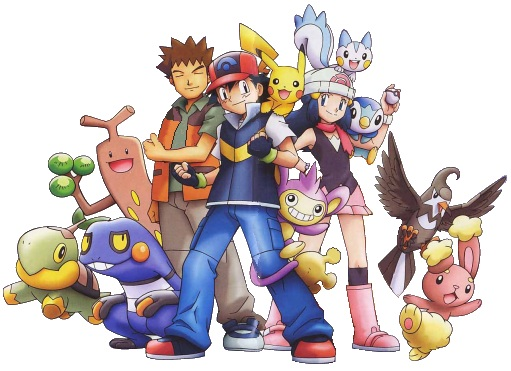
\includegraphics[width=0.5\linewidth]{pokemon.jpg}

    For when you just Gotta Catch 'Em All.
    \inputminted[linenos=false, numbersep=5pt, tabsize=4, fontsize=\tiny, firstline=5, lastline=9]{java}{singleLines.java}
\end{frame}

\begin{frame}{Anti-Pattern: Pokémon Exception Handling}
    Niemals Pokémon Exception Handling anwenden!
    \begin{itemize}[<+->]
        \item Die Fehlerbehandlung mit \myCode{catch} wird verwendet,
              um den Programmablauf nach einem Fehler zu definieren
        \item Bei unterschiedlichen Fehlern will man meist unterschiedlich
              weiter machen, z.B.
            \begin{itemize}
                \item IOException: nochmals versuchen
                \item NullPointerException: Fehlerbericht an den Entwickler schicken
                \item IllegalArgumentException: Fehlerausgabe an den Nutzer
            \end{itemize}
        \item Durch die verschiedenen \myCode{catch}-Blöcke zeigst du,
              dass du an die verschiedenen Fehlerarten gedacht hast
    \end{itemize}
\end{frame}

\begin{frame}{Größe des try-Blocks}
    \begin{block}{Wichtig}
        Der try-Block sollte so klein wie möglich sein.
    \end{block}

    Gründe:
    \begin{itemize}
        \item Beim lesen eures Codes wird klarer, wo das Problem
              auftreten kann
        \item Effizienz
    \end{itemize}
\end{frame}

\begin{frame}{Eigene Exceptions}
    \inputminted[linenos=true, numbersep=5pt, tabsize=4, fontsize=\small, label=UniverseExplodeException.java, frame=lines]{java}{UniverseExplodeException.java}
\end{frame}

\begin{frame}{@throws und throws}
    \begin{itemize}
        \item Exceptions, die nicht von RuntimeException erben, müssen angekündigt werden
        \item Ankündigen funktioniert über JavaDoc-Annotation \myCode{@throws} und Methodensignatur mit \myCode{throws}
    \end{itemize}

   \inputminted[linenos=false, numbersep=5pt, tabsize=4, fontsize=\small, firstline=11, lastline=21]{java}{singleLines.java}
\end{frame}

\subsection{Literatur}
\begin{frame}{Literatur}
    \begin{itemize}
        \item \href{http://docs.oracle.com/javase/tutorial/essential/exceptions/handling.html}{Catching and Handling Exceptions}
        \item \href{http://docs.oracle.com/javase/specs/jls/se7/html/jls-14.html\#jls-14.20}{JLS 7, Kapitel 14.20}
    \end{itemize}
\end{frame}

\section{Praxis}
\subsection{Türme von Hanoi}
\begin{frame}{Türme von Hanoi: Beschreibung}
    Das Spiel besteht aus drei Stäben A, B und C, auf die mehrere gelochte Scheiben gelegt werden,
    alle verschieden groß.\\
    Zu Beginn liegen alle Scheiben auf Stab A, der Größe nach geordnet, mit der
    größten Scheibe unten und der kleinsten oben.\\
    Ziel des Spiels ist es, den kompletten Scheiben-Stapel
    von A nach C zu versetzen.\\
    Bei jedem Zug darf die oberste Scheibe eines beliebigen Stabes auf einen
    der beiden anderen Stäbe gelegt werden, vorausgesetzt, dort liegt nicht schon eine kleinere Scheibe.
    Folglich sind zu jedem Zeitpunkt des Spieles die Scheiben auf jedem Feld der Größe nach geordnet.
\end{frame}

\begin{frame}{Aufgaben}
    \begin{block}{Klasse "`Disc"'}
        Schreiben Sie zunächst eine Klasse Disc, die eine gelochte
        Scheibe repräsentiert und als Attribut einen Durchmesser hat.
    \end{block}

    \begin{block}{Klasse "`Pole"'}
        Schreiben Sie außerdem eine Klasse Pole, die einen Stab repräsentiert. Ein solcher Stab verwaltet eine
        Menge von Discs (in einem fest dimensionierten Array) und hat als Attribut einen Namen. Die Klasse
        Pole stellt dabei sicher, dass die Scheiben immer in geordneter Reihenfolge (wie oben beschrieben)
        auf dem Stab liegen. Hierfür stellt die Klasse Pole die Methoden
        \myCode{public boolean push(Disc d)} und
        \myCode{public Disc pop()} zur Verfügung.
    \end{block}
\end{frame}

\begin{frame}{Aufgaben}
    \begin{block}{Methode push}
        Die Methode push(Disc d) legt die Scheibe d auf den Stab,
        falls dieser noch nicht voll ist und
        der Durchmesser der Scheibe d kleiner ist als der Durchmesser
        der obersten Scheibe des Stabes. Wird
        die Scheibe erfolgreich auf den Stab gelegt, so ist der
        Rückgabewert der Methode true, andernfalls
        false.
    \end{block}

    \begin{block}{Methode pop}
        Die Methode pop() entfernt die oberste Scheibe des Stabes und
        liefert diese als Rückgabewert. Falls
        der Stab leer ist, soll der Rückgabewert null sein.
    \end{block}

    Schreiben Sie, falls nötig, weitere Schnittstellen
    (z.B. eine Methode size()) und toString()-Methoden.
\end{frame}

\begin{frame}{Aufgaben}
    Eine weitere Klasse Hanoi soll die main-Methode und eine Methode mit der Signatur
    \myCode{public static void move(Pole from, Pole help, Pole to)}
    erhalten. Die Methode \myCode{move(Pole from, Pole help, Pole to)} legt dabei alle Scheiben das
    Stabes from mit Hilfe des Stabes help auf den Stab to. Implementieren Sie diese Methode rekursiv.
    Erzeugen Sie dann in der main-Methode einen Stab A mit mehreren Scheiben und zusätzlich zwei leere
    Stäbe B und C. Verwenden Sie dann die Methode move(), um die Scheiben von Stab A mit Hilfe des
    Stabes B auf Stab C zu legen.
\end{frame}

\section{Abspann}
\subsection{Klausuranmeldung}
\begin{frame}{Klausuranmeldung}
  Ist die Klausuranmeldung schon möglich? Bitte anmelden!
\end{frame}

\subsection{Kommende Tutorien}
\begin{frame}{Kommende Tutorien}
  \begin{itemize}
    \item[4.] 07.01.2013
    \item[3.] 14.01.2013
    \item[2.] 21.01.2013
    \item[1.] 28.01.2013: Abschlussprüfunsvorbereitung
    \item[0.] 04.02.2013: Abschlussprüfunsvorbereitung
    \item[-] 10.02.2013: Ende der Vorlesungszeit des WS 2012/2013 (\href{http://www.kit.edu/studieren/2873.php}{Quelle})
  \end{itemize}
\end{frame}

\framedgraphic{Vielen Dank für eure Aufmerksamkeit!}{../images/Teach-yourself-C++-in-21-days.png}

\end{document}
